

\tikzset{every picture/.style={line width=0.75pt}} %set default line width to 0.75pt        

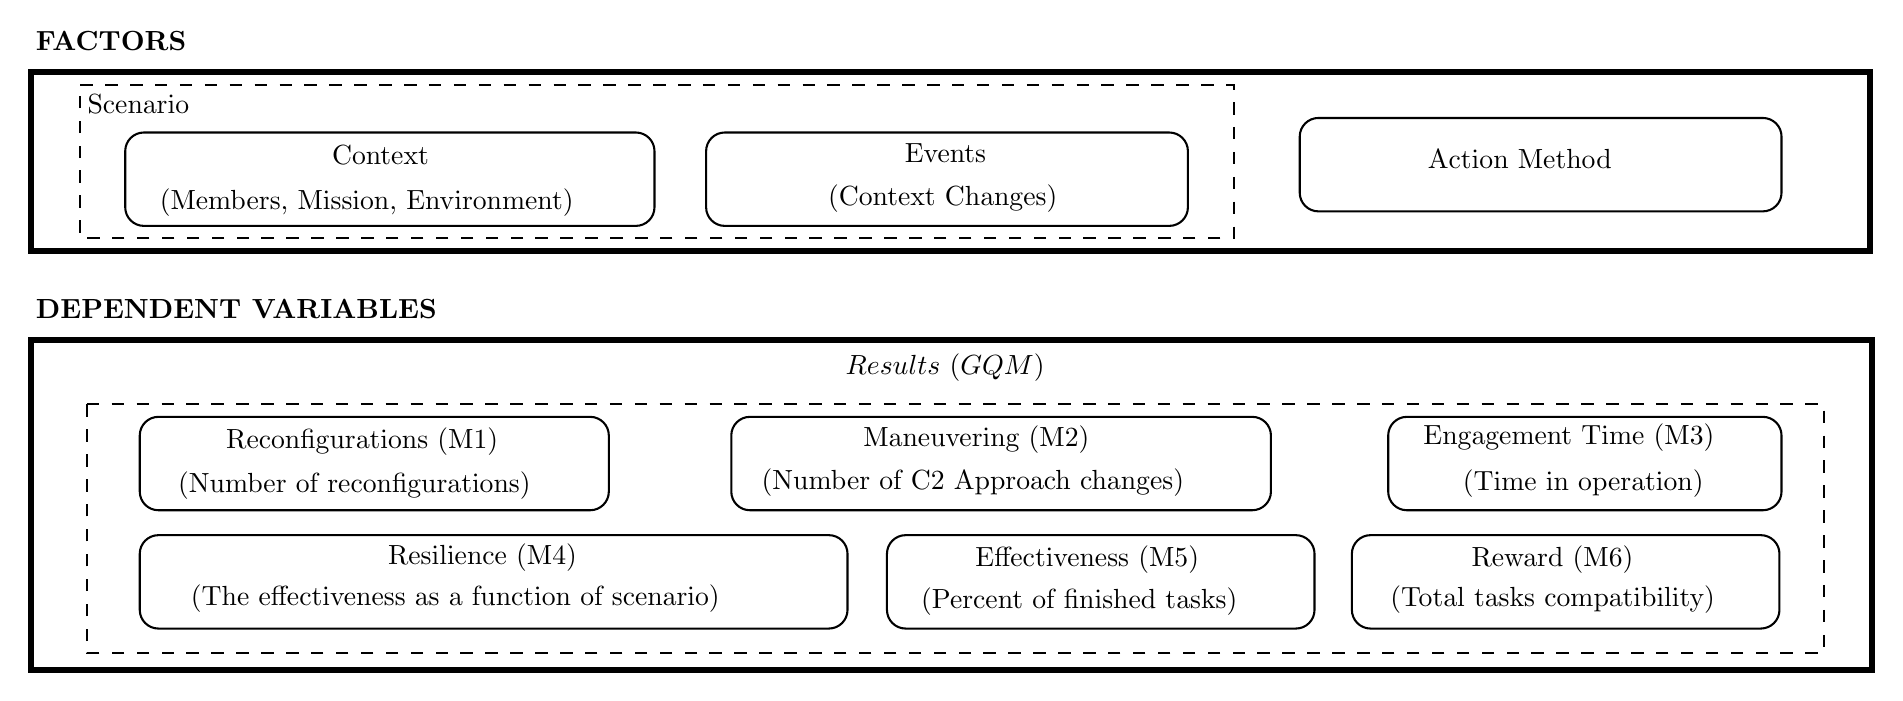
\begin{tikzpicture}[x=0.75pt,y=0.75pt,yscale=-1,xscale=1]
%uncomment if require: \path (0,322); %set diagram left start at 0, and has height of 322

%Rounded Rect [id:dp26709545620813635] 
\draw   (57.5,200) .. controls (57.5,195.03) and (61.53,191) .. (66.5,191) -- (274.5,191) .. controls (279.47,191) and (283.5,195.03) .. (283.5,200) -- (283.5,227) .. controls (283.5,231.97) and (279.47,236) .. (274.5,236) -- (66.5,236) .. controls (61.53,236) and (57.5,231.97) .. (57.5,227) -- cycle ;
%Shape: Rectangle [id:dp7868821488097882] 
\draw  [dash pattern={on 4.5pt off 4.5pt}] (32,185) -- (869,185) -- (869,305) -- (32,305) -- cycle ;
%Shape: Rectangle [id:dp07661178173797467] 
\draw  [line width=2.25]  (5,153.88) -- (892,153.88) -- (892,313) -- (5,313) -- cycle ;
%Rounded Rect [id:dp7819847156561298] 
\draw   (50.5,63) .. controls (50.5,58.03) and (54.53,54) .. (59.5,54) -- (296.5,54) .. controls (301.47,54) and (305.5,58.03) .. (305.5,63) -- (305.5,90) .. controls (305.5,94.97) and (301.47,99) .. (296.5,99) -- (59.5,99) .. controls (54.53,99) and (50.5,94.97) .. (50.5,90) -- cycle ;
%Shape: Rectangle [id:dp10398748207162001] 
\draw  [dash pattern={on 4.5pt off 4.5pt}] (28.85,31) -- (584.5,31) -- (584.5,105) -- (28.85,105) -- cycle ;
%Shape: Rectangle [id:dp48323694433186415] 
\draw  [line width=2.25]  (5,24.77) -- (891,24.77) -- (891,111) -- (5,111) -- cycle ;
%Rounded Rect [id:dp14086907660692627] 
\draw   (330.37,63) .. controls (330.37,58.03) and (334.4,54) .. (339.37,54) -- (553.5,54) .. controls (558.47,54) and (562.5,58.03) .. (562.5,63) -- (562.5,90) .. controls (562.5,94.97) and (558.47,99) .. (553.5,99) -- (339.37,99) .. controls (334.4,99) and (330.37,94.97) .. (330.37,90) -- cycle ;
%Rounded Rect [id:dp8800855997802748] 
\draw   (616.37,56) .. controls (616.37,51.03) and (620.4,47) .. (625.37,47) -- (839.5,47) .. controls (844.47,47) and (848.5,51.03) .. (848.5,56) -- (848.5,83) .. controls (848.5,87.97) and (844.47,92) .. (839.5,92) -- (625.37,92) .. controls (620.4,92) and (616.37,87.97) .. (616.37,83) -- cycle ;
%Rounded Rect [id:dp41591552385229413] 
\draw   (659,200) .. controls (659,195.03) and (663.03,191) .. (668,191) -- (839.5,191) .. controls (844.47,191) and (848.5,195.03) .. (848.5,200) -- (848.5,227) .. controls (848.5,231.97) and (844.47,236) .. (839.5,236) -- (668,236) .. controls (663.03,236) and (659,231.97) .. (659,227) -- cycle ;
%Rounded Rect [id:dp6557542326475674] 
\draw   (342.5,200) .. controls (342.5,195.03) and (346.53,191) .. (351.5,191) -- (593.5,191) .. controls (598.47,191) and (602.5,195.03) .. (602.5,200) -- (602.5,227) .. controls (602.5,231.97) and (598.47,236) .. (593.5,236) -- (351.5,236) .. controls (346.53,236) and (342.5,231.97) .. (342.5,227) -- cycle ;
%Rounded Rect [id:dp018207773722970888] 
\draw   (641.5,257) .. controls (641.5,252.03) and (645.53,248) .. (650.5,248) -- (838.5,248) .. controls (843.47,248) and (847.5,252.03) .. (847.5,257) -- (847.5,284) .. controls (847.5,288.97) and (843.47,293) .. (838.5,293) -- (650.5,293) .. controls (645.53,293) and (641.5,288.97) .. (641.5,284) -- cycle ;
%Rounded Rect [id:dp7136990985847002] 
\draw   (57.5,257) .. controls (57.5,252.03) and (61.53,248) .. (66.5,248) -- (389.5,248) .. controls (394.47,248) and (398.5,252.03) .. (398.5,257) -- (398.5,284) .. controls (398.5,288.97) and (394.47,293) .. (389.5,293) -- (66.5,293) .. controls (61.53,293) and (57.5,288.97) .. (57.5,284) -- cycle ;
%Rounded Rect [id:dp3168441468736909] 
\draw   (417.5,257) .. controls (417.5,252.03) and (421.53,248) .. (426.5,248) -- (614.5,248) .. controls (619.47,248) and (623.5,252.03) .. (623.5,257) -- (623.5,284) .. controls (623.5,288.97) and (619.47,293) .. (614.5,293) -- (426.5,293) .. controls (421.53,293) and (417.5,288.97) .. (417.5,284) -- cycle ;

% Text Node
\draw (396.1,159.07) node [anchor=north west][inner sep=0.75pt]    {$Results\ ( GQM)$};
% Text Node
\draw (6,133) node [anchor=north west][inner sep=0.75pt]   [align=left] {\textbf{DEPENDENT VARIABLES}};
% Text Node
\draw (148.64,58.62) node [anchor=north west][inner sep=0.75pt]   [align=left] {Context};
% Text Node
\draw (6,4) node [anchor=north west][inner sep=0.75pt]   [align=left] {\textbf{FACTORS}};
% Text Node
\draw (65.64,79.62) node [anchor=north west][inner sep=0.75pt]   [align=left] {(Members, Mission, Environment)};
% Text Node
\draw (424.64,57.62) node [anchor=north west][inner sep=0.75pt]   [align=left] {Events};
% Text Node
\draw (387.64,77.62) node [anchor=north west][inner sep=0.75pt]   [align=left] {(Context Changes)};
% Text Node
\draw (676.64,60.62) node [anchor=north west][inner sep=0.75pt]   [align=left] {Action Method};
% Text Node
\draw (693.5,215) node [anchor=north west][inner sep=0.75pt]   [align=left] {(Time in operation)};
% Text Node
\draw (674.5,193) node [anchor=north west][inner sep=0.75pt]   [align=left] {Engagement Time (M3)};
% Text Node
\draw (30.85,34) node [anchor=north west][inner sep=0.75pt]   [align=left] {Scenario};
% Text Node
\draw (74.5,216) node [anchor=north west][inner sep=0.75pt]   [align=left] {(Number of reconfigurations)};
% Text Node
\draw (97.64,194.62) node [anchor=north west][inner sep=0.75pt]   [align=left] {Reconfigurations (M1)};
% Text Node
\draw (355.64,214.62) node [anchor=north west][inner sep=0.75pt]   [align=left] {(Number of C2 Approach changes)};
% Text Node
\draw (404.64,193.62) node [anchor=north west][inner sep=0.75pt]   [align=left] {Maneuvering (M2)};
% Text Node
\draw (658.5,271) node [anchor=north west][inner sep=0.75pt]   [align=left] {(Total tasks compatibility)};
% Text Node
\draw (697.64,251.62) node [anchor=north west][inner sep=0.75pt]   [align=left] {Reward (M6)};
% Text Node
\draw (80.64,270.62) node [anchor=north west][inner sep=0.75pt]   [align=left] {(The effectiveness as a function of scenario)};
% Text Node
\draw (175.64,250.62) node [anchor=north west][inner sep=0.75pt]   [align=left] {Resilience (M4)};
% Text Node
\draw (432.5,272) node [anchor=north west][inner sep=0.75pt]   [align=left] {(Percent of finished tasks)};
% Text Node
\draw (458.64,251.62) node [anchor=north west][inner sep=0.75pt]   [align=left] {Effectiveness (M5)};


\end{tikzpicture}